\documentclass[../mathNotesPreamble]{subfiles}

\providecommand{\relscalefact}{1.4}
\begin{document}
\relscale{\relscalefact}
  \section{2.3: Visualizing Variation in Categorical Variables}
  \begin{defn*}
    A \textbf{bar chart} (also bar graph or bar plot) shows a bar for each observed category where the height of the bar is proportional to the frequency of that category.
  \end{defn*}
  \begin{ex*}
    A summer introductory statistics course at UCLA has the following distribution of students across different years:
  \end{ex*}

  \noindent
  \begin{minipage}{0.3\linewidth}
    \begin{center}
      \begin{tabular}{@{}lr@{}}\toprule
        Class& Frequency\\\midrule
        Unknown& 7\\
        Freshman& 0\\
        Sophomore& 3\\
        Junior& 4\\
        Senior& 5\\
        Graduate& 1\\\midrule
        Total& 20\\\bottomrule
      \end{tabular}
    \end{center}
  \end{minipage}%
  \hspace*{\stretch{1}}
  \begin{minipage}{0.625\linewidth}
    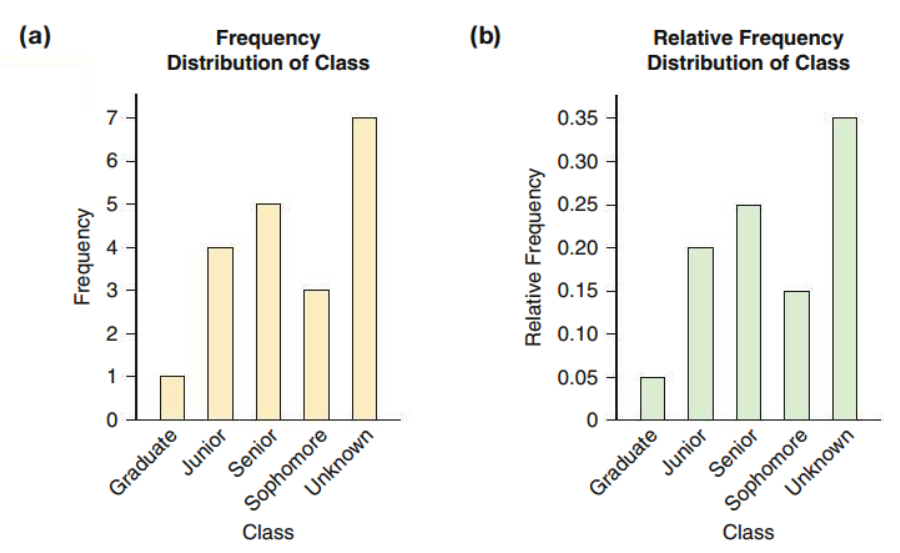
\includegraphics[width=\linewidth]{images/math211_figure_2p25}
  \end{minipage}
  \vspace*{\stretch{1}}

  \noindent
  \fbox{\parbox{0.9875\linewidth}{
    \textbf{Bar Charts vs. Histograms:}
    \begin{tasks}[label=\textbullet](2)
      \task Histograms are for numerical data
      \task Bar charts are for categorical data
    \end{tasks}
    \begin{center}
      \begin{tabular}{@{}rll@{}}\toprule
        & Histogram& Bar Chart\\\midrule
        Bars: & Should touch& May or may not touch\\
        Bar width: & Corresponds to bin width & Can be any width (consistent)\\
        Horizontal labels: & Numerical order& No inherent order\\\bottomrule
      \end{tabular}
    \end{center}
    \begin{itemize}
      \item A \textbf{Pareto chart} is a bar graph with bars arranged from tallest to shortest.
    \end{itemize}
  }}
  \pagebreak

  \begin{defn*}
    A \textbf{pie chart} is a circle divided up into pieces where each area is proportional to the relative frequency of the category it represents.
  \end{defn*}
  \begin{ex*}

  \end{ex*}
  \noindent
  \hspace*{\stretch{1}}
  \begin{minipage}{0.3\linewidth}
    \begin{center}
      \begin{tabular}{@{}lr@{}}\toprule
        Class& Frequency\\\midrule
        Unknown& 7\\
        Freshman& 0\\
        Sophomore& 3\\
        Junior& 4\\
        Senior& 5\\
        Graduate& 1\\\midrule
        Total& 20\\\bottomrule
      \end{tabular}
    \end{center}
  \end{minipage}%
  \hspace*{\stretch{1}}
  \begin{minipage}{0.3\linewidth}
    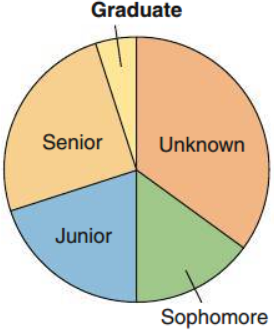
\includegraphics[width=\linewidth]{images/math211_figure_2p27}
  \end{minipage}
  \hspace*{\stretch{1}}



  \pagebreak
\end{document}
